\chapter{EEXCESS-Browser}

\section{Lesezeichen hinzufügen}
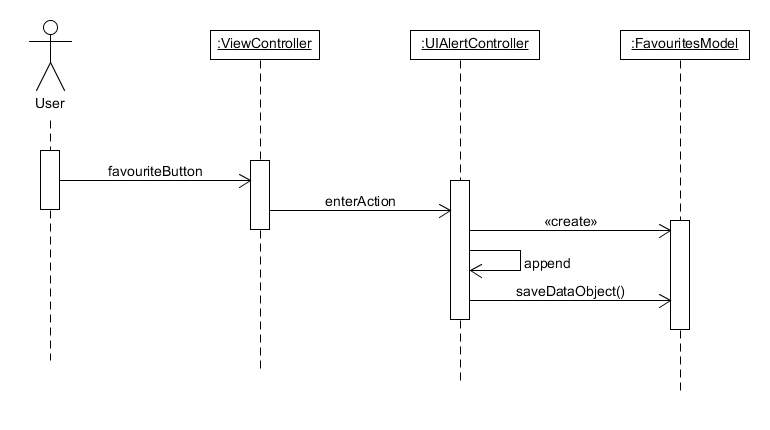
\includegraphics[scale=0.5]{sequAddFavourites.png}
Nachdem der User auf den Plusbutton zum Hinzufügen eines neuen Lesezeichens klickt, wird im ViewController die IBAction des Buttons aufgerufen. Hier wird die enterAction des UIAlertControllers aufgerufen. Nun kann der Nutzer den gewünschten Titel des Lesezeichens eingeben. Die URL wird automatisch übernommen. Nachdem man auf Enter zum Bestätigen klickt, wird ein neues Objekt des FavouriteModels erzeugt. Anschließend wird das erstellte Lesezeichen in das Model geschrieben und persistent gespeichert.
\pagebreak

\section{Lesezeichen bearbeiten}
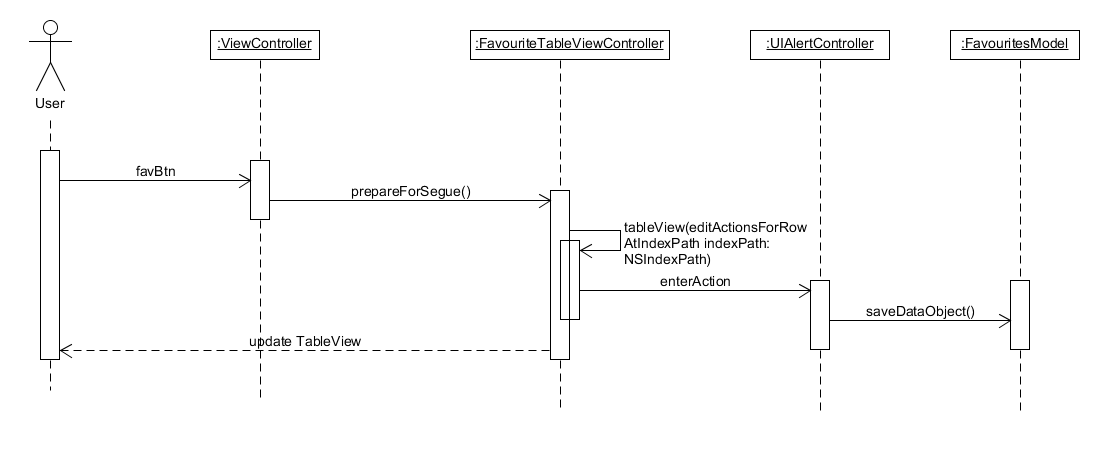
\includegraphics[scale=0.40]{sequEditFavourites.png}
Nachdem der User auf das Lesezeichensymbol zum Anzeigen der gespeicherten Lesezeichen klickt, wird im ViewController die prepareForSegue-Methode aufgerufen. Nun wird der FavouriteTableViewController geladen. Hier wird die Methode editActionsForRowAtIndexPath indexPath: NSIndexPath) aufgerufen. Nachdem man den entsprechenden Eintrag in der TableView auswählt, öffnet sich ein AlertFenster. Hier ist es möglich, den Titel zu ändern. Nach dem Bestätigen wird dies persistent gespeichert und die TableView aktualisiert.
\pagebreak

\section{Lesezeichen anzeigen}
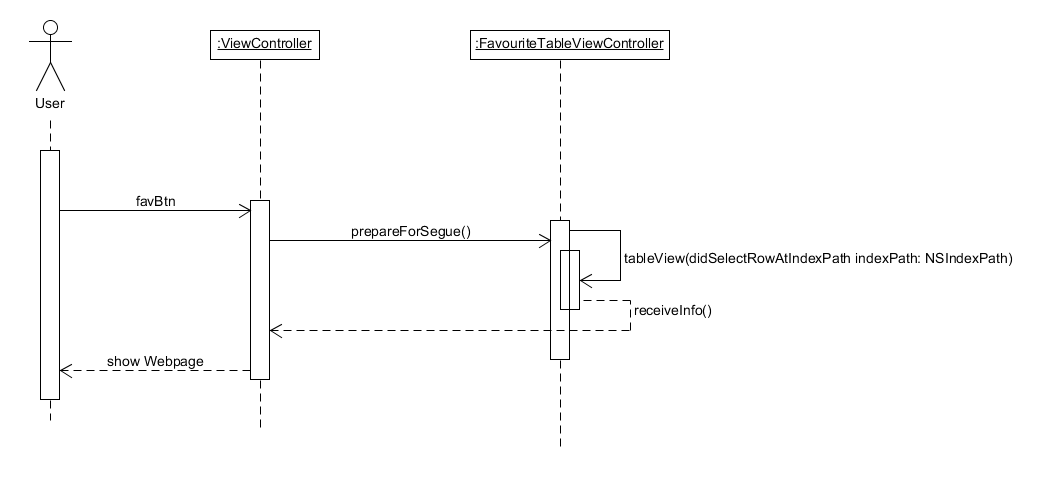
\includegraphics[scale=0.45]{sequShowFavourites.png}
Nachdem der User auf das Lesezeichensymbol zum Anzeigen der gespeicherten Lesezeichen klickt, wird im ViewController die prepareForSegue-Methode aufgerufen. Nun wird der FavouriteTableViewController geladen. Hier wird die Methode tableView(didSelectRowAtIndexPath indexPath: NSIndexPath) augerufen. Hier wird überprüft, ob der Nutzer auf eine Zelle der TableView geklickt hat. Sobald man auf eine Zelle klickt, wird die entsprechende URL im FavouriteModel gespeichert und die Delegate-Methode receiveInfo() im ViewController aufgerufen. Dort wird die Methode loadURL mit der entsprechenden URL aufgerufen. Anschließend gelangt der Nutzer zum ViewController und die URL wird in der WebView angezeigt.
\pagebreak

\section{Lesezeichen löschen}
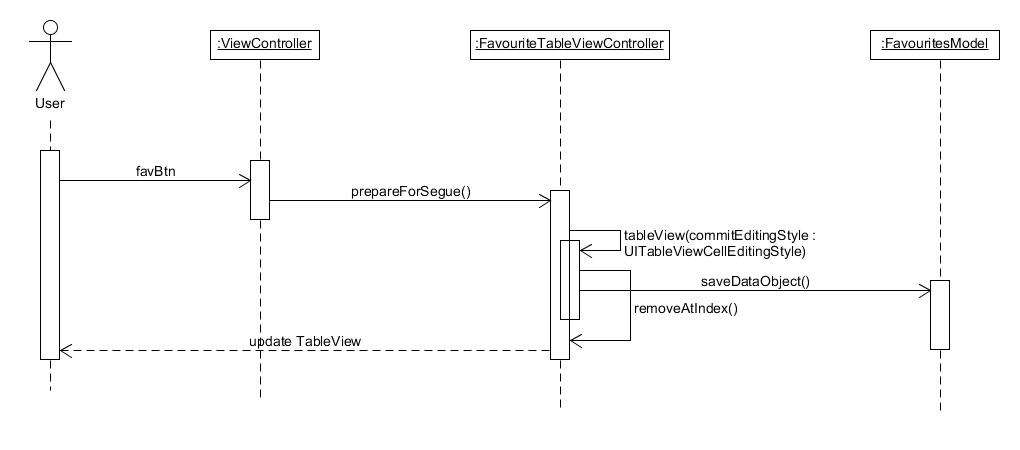
\includegraphics[scale=0.45]{sequDeleteFavourites.png}
Nachdem der User auf das Lesezeichensymbol zum Anzeigen der gespeicherten Lesezeichen klickt, wird im ViewController die prepareForSegue-Methode aufgerufen. Nun wird der FavouriteTableViewController geladen. Hier wird die Methode editActionsForRowAtIndexPath indexPath: NSIndexPath) aufgerufen. Hier wird der ausgewählte Eintrag gelöscht. Dies wird persistent gespeichert und die TableView aktualisiert.
\pagebreak
